\documentclass[10pt]{article}

%% Packages %%
\usepackage{hyperref}  % links
\usepackage{graphicx}  % images
\usepackage{listings}  % code
\usepackage{authblk}  % author info
\usepackage{biblatex}  % bibliography
\usepackage[utf8]{inputenc}
\addbibresource{rhel_source.bib}

%% Preamble %%
%% Metadata %%
\title{Centos Operating sytem Security application}

\author{Truong PhaT Tu}
\affil{
Luther College\\
Decorah, IA 52101\\
tuph01@luther.edu
}

\date{\today}

%% Document body %%
\begin{document}

%% Abstract. Must be before \maketitle is called %%


\maketitle

\tableofcontents

\section{Introduction}

Vietnamese version cs296
Introduction
The operating system is known as a support platform to help interact with your applications and assist users with appropriate tasks. The operating system is tailored to the needs and tasks, in which the operating system for the server is customized to interact and receive information and process them with high intensity, and in which the operating systems are customized. Typically used for servers, used for businesses are individually tailored and processed to be able to handle multiple objects interacting with the server at the same time. Since tasks are used to receive large amounts of information, process and return large amounts of information, and hold important business and user information, stability and security are important parts of a system. operating. In which the security of an operating system is treated specifically and its importance is so in the operating systems used for the server used, Centos OS is one of them with the application of security in the operating system for the server. And to explain the safety of this operating system will be explained preliminary, note that the research may not be completely correct and there will be errors in the research process because there is no money to have the necessary information. articles, research articles. The study is divided into 3 main parts including, the history of the Centos operating system, the RHEL source code used as a source of code for linux O strong Centos, the capability and security of the system. operating based on the above. At the same time, the source of RHEL's code and its ability to report security against hackers and vulnerabilities are patched after a period of time.

History
Centos OS is a used operating system and is quite popular when applied to enterprise servers. According to Wikipedia Centos was programmed with the first version with Centos ver 2 in 2004 and developed based on RHEL version 2 1SA used in this operating system until version 8 has been upgraded and adjusted for the chip generation with a 64x architecture to support hardware with existing and developed architectures, improving performance. The performance of the hardware and applications is used in an interoperable manner, and the information resources are processed faster, more efficiently, and more securely.

\section{History of the subject}
\subsection{Centos}


CentOS, an enterprise Linux distribution, was created by the CentOS Project community using the source code of Redhat Enterprise Linux (RHEL) as a free alternative to RHEL. It was designed to be as stable and compatible as its commercial counterpart, making it an ideal choice for learning Linux. Since CentOS was built using RHEL's source code, it is binary compatible with it, and the developers made sure to follow RHEL's redistribution rules, making it a genuinely free alternative. CentOS is continuously being developed by its core developers and community to ensure its stability through security and software updates, quality assurance measures, and release upgrades to support new hardware and software. The CentOS community is interactive, and users can seek assistance and share ideas through the community's website. Business users can also avail commercial support for CentOS through companies that specialize in it.
\cite{CentosAbout}

\subsection{RHEL}

We’re the world’s leading provider of enterprise open source solutions—including Linux, cloud, container, and Kubernetes. We deliver hardened solutions that make it easier for enterprises to work across platforms and environments, from the core datacenter to the network edge.
\cite{RHELAbout}
One of the main features of CentOS is its use of open source code from Red Hat Enterprise Linux (RHEL). RHEL distributes this open source code freely for use in operating systems, starting from version 2. CentOS is built from the open source code of RHEL, and is developed using the C++ programming language.

\section{Prominent features}

\subsection{Security in Centos OS}
Regarding security for CentOS operating system, it is divided into two types of security, including local security and network security. Local security is divided into two sub-branches (basic, advanced). The purpose of this division is to aim at different types of security. Since CentOS is often used for server operating systems and basic usage, it is always necessary to have the most basic security platforms to protect devices from intrusions and to control users when connecting to servers.

\subsubsection*{Basic security}
The system logger is important and necessary for every operating system to be able to record activities. Not only that, it also logs other types such as cron commands. These logs will be stored with the syntax: 
\newline\newline 
Date time host name message
\newline\newline 
This basic information is logged when an event occurs and is used to clearly identify information about the action through the messages, thereby assisting in early detection of intrusions from an unknown party and enhancing the security of the server being used.
\cite{FoCL}

\begin{figure}[!htbp]
    \centering
    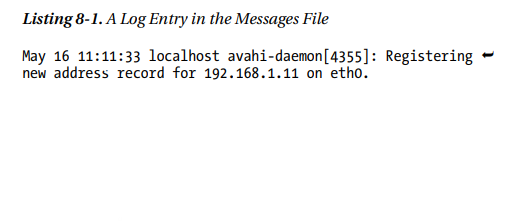
\includegraphics[width=0.4\textwidth]{./research_example/Screenshot 2023-04-26 220656.png}
    \begin{description}
        \item[] 
    \end{description}
    \caption{A log Entry in the messages file}
    \label{fig:description}
\end{figure}

\subsubsection{Automating task with Cron}
For crontab, it is use for some specific case , If you're managing other server software packages that hold sensitive data, such as database and file servers, it's crucial to protect them. Regular backups of these computers are necessary to ensure the data is retrievable in case of server failure. However, manually creating backups at specific times can be cumbersome and prone to errors, such as forgetting to create one. To simplify this process, CentOS offers a crontab command that automates tasks.
\cite{FoCL}

\subsubsection{Pluggable Authentication Modules}
To protect the server in identifying user accounts, CentOS is divided into two ways to authenticate accounts, using SSH and Cron Daemon.
\newline There are many ways to authenticate users in Linux applications, from using usernames and passwords to using certificates and keys to protect information. These have their own strengths and weaknesses. Because security features support data protection for administrators, applications provide security mechanisms that differ in authentication and user access.
\cite{FoCL}
\begin{figure}[!htbp]
    \centering
    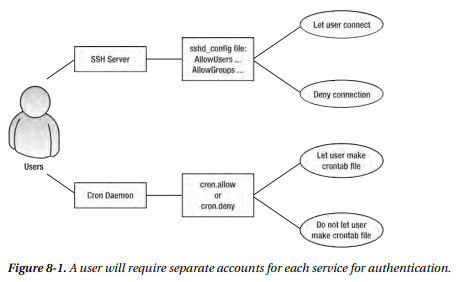
\includegraphics[width=0.4\textwidth]{./research_example/Screenshot 2023-04-14 122628.png}
    \begin{description}
        \item[] 
    \end{description}
    \caption{A user will require separate accounts for each service for authentication.}
    \label{fig:description}
\end{figure}
\newline Linux-PAM is widely used by Linux-based systems, including CentOS, to handle user authentication, session management, and password policies. Its pluggable nature allows system administrators to add or remove authentication modules without modifying the core system.
\begin{figure}[!htbp]
    \centering
    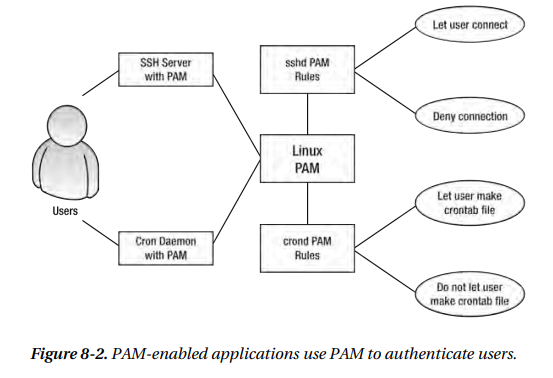
\includegraphics[width=0.4\textwidth]{./research_example/Screenshot 2023-04-26 235210.png}
    \begin{description}
        \item[] 
    \end{description}
    \caption{PAM-enabled applications use PAM to authenticate users.}
    \label{fig:description}
\end{figure}
\newline To avoid conflicts among applications on the operating system, CentOS developed Linux-Pam as an intermediate library that supports various methods of account authentication in applications, helping to minimize conflicts that can lead to security vulnerabilities in applications on the operating system.
\cite{FoCL}


\subsubsection{Advance Security}

\subsubsection{Network security}

\subsection{application of RHEL in Centos}

In CentOS operating system, the use of the source code from Red Hat is implemented to enhance and protect the system from manual attacks such as USB attacks. To prevent data breaches from the server and protect the system being used, CentOS OS uses USBGuard from RHEL source code to avoid attacks such as spyware, malware, or trojan. By using USBGuard, the operating system can prevent and authorize USB devices, as well as modify access rights to USB devices with the OS. This enables the device running CentOS OS to avoid intrusion from other devices and indirectly receive malicious codes.
\cite{RHEL9Sh}

\begin{figure}[!htbp]
        \centering
        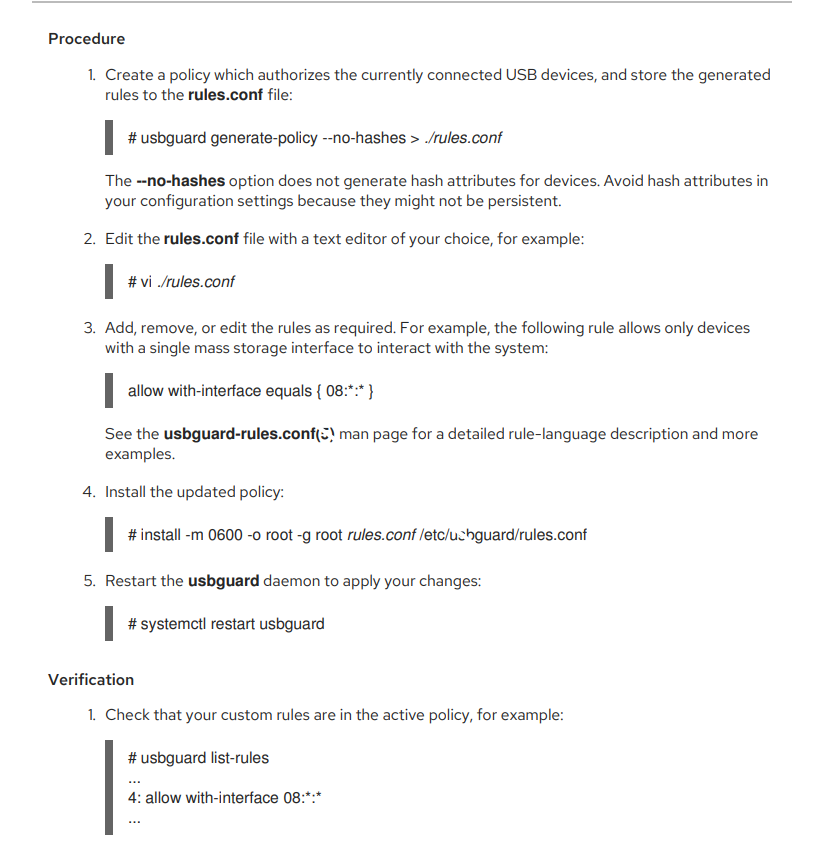
\includegraphics[width=0.4\textwidth]{./research_example/Screenshot 2023-04-21 163515.png}
        \begin{description}
            \item[] 
        \end{description}
        \caption{CREATING A CUSTOM POLICY FOR USB DEVICES}
        \label{fig:description}
    \end{figure}

Furthermore, CentOS is often used for Linux applications that require real-time performance or for system servers. CentOS has a relatively longer support and release cycle, leading to a highly stable system. However, security hardening technology is also important.

"The initial basis for generating hardening scripts used within the proposed framework
has been expanded on from Frank Caviggia’s CentOS 7 project used for a standard 
distribution that is not capable of real-time performance [8]. Caviggia developed these 
scripts while working at Red Hat and along with others in the community continues to 
maintain them. The primary goal of Caviggia’s scripts is to configure and harden the 
baseline CentOS ISO using SCAP Security Guide (SSG). Red Hat maintains a RHEL 
based fork of Caviggia’s project [9]. The security hardening is implemented using 
RHEL’s standard kickstart technology."
\cite{ALSHHfRtAR_SCAP_C}


\cite{SEiRHEL}
\subsection{unknown}
In terms of security, as an open source operating system, CentOS is developed and audited by a large community, which enhances its safety. Additionally, the OS supports the Security Content Automation Protocol (SCAP), which helps protect against cyberattacks. It also supports monitoring and logging to detect any device activity and defend against attacks.
\section{Conclusion}

\begin{figure}[!htbp]
    \centering
    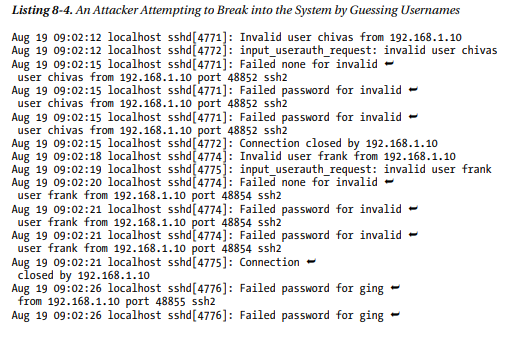
\includegraphics[width=0.4\textwidth]{./research_example/Screenshot 2023-04-14 122536.png}
    \begin{description}
        \item[] 
    \end{description}
    \caption{4. An Attacker Attempting to Break into the System by Guessing Usernames }
    \label{fig:description}
\end{figure}
%% Bibliography. Must be just before the end of the document %%
\printbibliography

\end{document}